\documentclass{article}
\usepackage{color}
\usepackage[backref,colorlinks,linkcolor=black,urlcolor=blue]{hyperref}
\usepackage{graphicx}
\usepackage{float}
\usepackage{ctex}
\usepackage{tabularx}
\usepackage{geometry}
\usepackage{listings}
\usepackage{fontspec}
\usepackage{indentfirst}

\setlength{\parindent}{2em}
\geometry{a4paper,left=3cm,right=3cm,top=3.5cm,bottom=3.5cm}
\lstset{
    basicstyle={\fontspec{Consolas} \small},
    breaklines=true,
    keywordstyle={\color{red} \fontspec{Consolas Bold}},
    commentstyle={\color[RGB]{30,120,30} \fontspec{Consolas Italic}},
    tabsize=4
}

\begin{document}

% cover begin

\thispagestyle{empty}
\setcounter{page}{-1}

\begin{center}
    
\includegraphics[width=0.5\paperwidth]{logo.png}
\end{center}

\vskip 20pt

\begin{center}
    \zihao{3}
    \textbf{本科实验报告}
\end{center}


\vskip 120pt

    \begin{center}
        \bfseries \zihao{-2}

        \begin{tabularx}{.7\textwidth}{>{\fangsong}l >{\fangsong}X<{\centering}}
            课程名称 & \uline{\hfill 编译原理 \hfill} \\
            姓名 &  \uline{\hfill  \hfill} \\
            学院 &  \uline{\hfill  \hfill} \\
            专业 &  \uline{\hfill  \hfill} \\
            学号 &  \uline{\hfill  \hfill} \\
            指导教师 &  \uline{\hfill  \hfill} \\
            ~ & ~\\
        \end{tabularx}
    \end{center}

\vskip 100pt

\begin{center}
    \zihao{3} \fangsong
    \today
\end{center}

% cover end


\newpage

\thispagestyle{empty}

\zihao{4}
\tableofcontents

\newpage

\zihao{-4}


\section*{序言}
\addcontentsline{toc}{section}{序言}

\subsection*{概述}
\addcontentsline{toc}{subsection}{概述}
\par 本项目是SPL——一门Pascal的方言——的编译器工程,使用Flex进行词法分析,Bison进行语法分析,通过构建抽象语法树,使用LLVM API生成LLVM IR,再由LLVM框架将平台无关的中间码转换至对应平台的汇编代码,并编译为可执行的二进制文件。
\par 本项目使用 \href{https://github.com/uninstalle/SPLCompiler}{github} 托管。

\subsection*{编译环境}
\addcontentsline{toc}{subsection}{编译环境}
\begin{itemize}
    \item Prebuilt environment: Linux Ubuntu 20.04
    \item Lexer: flex 2.6.4
    \item Parser: bison 3.5.1
    \item Framework: LLVM 12.0.0
\end{itemize}

\subsection*{文件结构}
\addcontentsline{toc}{subsection}{文件结构}
\begin{lstlisting}
Root
│  build.sh  //编译compiler
│  clean.sh  //清理产生的compiler及中间文件
│  run.sh  //运行compiler并将产生的LLVM IR编译为可执行文件
│
├─bin
│  └─ main  //预编译的compiler
├─src
│  │  main.cc  //入口
│  │  Parser.cc  //bison产生的中间文件
│  │  Parser.hh  //bison产生的中间文件
│  │  Scanner.cc  //flex产生的中间文件
│  │
│  ├─ast
│  │      ast.hh  //include-all header
│  │      ast_base.cc
│  │      ast_base.hh //基类node
│  │      ast_const.cc
│  │      ast_const.hh  //常量node,包含各种常量从token到llvm::Value的转换
│  │      ast_expr.cc
│  │      ast_expr.hh  //表达式node,包含表达式中会出现的所有token的解析
│  │      ast_function.cc
│  │      ast_function.hh  //函数node,包含函数的声明与定义
│  │      ast_routine.cc
│  │      ast_routine.hh  //例程node,包含routine和subroutine的实现
│  │      ast_stmt.cc
│  │      ast_stmt.hh  //语句node,包含赋值、流程控制、过程调用等
│  │      ast_type.cc
│  │      ast_type.hh  //类型node,包含类型的解析和从token到llvm::Type的转换
│  │      ast_variable.cc
│  │      ast_variable.hh  //变量node,包含变量的定义与内存分配
│  │
│  ├─irgen
│  │      generator.cc
│  │      generator.hh  //AST的操作者,实现AST的生成、AST的输出、IR的生成
│  │      table.cc
│  │      table.hh  //符号表的定义
│  │
│  ├─lexer
│  │      Scanner.l  //词法分析器
│  │
│  ├─logger
│  │      logger.cc
│  │      logger.hh  //输出log的工具
│  │
│  └─parser
│         Parser.yy  //语法分析器
│
└─test
        test1.spl  //基本语句的测试
        test2.spl  //给定test
        test2ans.cc  //给定test的c++转写,用于测试结果
        test3.spl  //IO测试
        test4.spl  //给定test
        test4ans.cc
        test5.spl  //数组与记录的使用,函数引用传递的测试
        test6.spl  //给定test
        test6ans.cc

\end{lstlisting}

\subsection*{使用说明}
\addcontentsline{toc}{subsection}{使用说明}
\begin{enumerate}
  \item 运行build.sh。该操作将会产生src/目录下的Scanner.cc,Parser.hh,Parser.cc文件以及bin/下的可执行文件main,即SPL的编译器。main接受两个参数:目标文件的路径,(可选)任意字符(用于启动优化)。未提供第二个参数时仅进行最基本的优化(如常量折叠),提供后将额外进行LLVM API提供的几项优化。main在执行后会产生以下文件:
    \begin{itemize}
      \item lex.log:记录lexer解析时关键字以外的内容,例如name、常量等。
      \item yacc.log:记录分析得到的抽象语法树。节点关系以缩进表示。
      \item codegen.log:记录生成中间代码过程中的额外信息,用于debug。
      \item out.ll:运行结果,产生的LLVM IR。
    \end{itemize}
  \item 运行run.sh。run.sh的两个参数将在调用main时转发给main。该脚本在完成LLVM IR的生成后还将通过clang将LLVM IR编译为二进制文件并执行。
\end{enumerate}

\subsection*{分工说明\&总览}
\addcontentsline{toc}{subsection}{总览}

\begin{table}[H]
    \begin{tabular}{|l|l|l|l|}
        \hline
        \textbf{Compiler Component}    & \textbf{Status} & \textbf{Details}   & \textbf{Coder}  \\ \hline
        Scanning                       & Flex            &                    &           \\ \hline
        Parsing                        & Bison           &                    &           \\ \hline
        Semantic Analysis              & AST             &                    &           \\ \hline
        Intermediate Code Generation   & LLVM IR         & LLVM IRBuilder     &           \\ \hline
        Intermediate Code Optimization & LLVM C++ API    & LLVM Pass Manager  &           \\ \hline
        Target Code Generation         & LLVM back-end   & Clang++            &           \\ \hline
        Target Code Optimization       & LLVM back-end   & Clang++            &           \\ \hline
        Other Optimization             & implemented     &                    &           \\ \hline
        Runtime Environment            & implemented     & 全局栈环境          &          \\ \hline
        Symbol Table                   & implemented     &                    &           \\ \hline
        Report                         &                 & Latex              &           \\ \hline
    \end{tabular}
\end{table}

\newpage
\section{词法分析}
\subsection{正则表达式}
\subsubsection{关键字}
\par 接受所有语言定义关键字的小写形式。
\subsubsection{运算符}
\par 接受所有语言定义运算符的数学符号形式。此外,与或非及求余在数学符号之外还支持大写字母表示(AND/OR/NOT/MOD)。
\subsubsection{标识符}
\par 标识符包含所有非关键字或系统占用的ID。系统使用ID(系统常量、系统子程序、系统函数等)将在全局空间预定义。
\par $ NAME = [a-zA-Z][\_a-zA-Z0-9]* $

\subsubsection{常量}
\begin{itemize}
  \item 整数 $ INTEGER = -?[0-9]+ $
  \item 实数 $ REAL = -?[0-9]+("."[0-9]+|e-?[0-9]+) $
  \item 字符 $ CHARACTER = '.' $
  \item 字符串 $ STRING = '[\^{}']\{0,255\}' $
\end{itemize}

\par 根据lex的最长优先匹配规则,实数将优先于整数匹配,因此不会出现整数匹配了实数的一部分这一问题。

\subsubsection{其他}

\begin{itemize}
  \item 空白字符 $ WHITE\_SPACE = [ \backslash t]+ $
  \item 未识别字符 $ UNRECOGNIZED = . $
\end{itemize}

\par 空白字符在捕获后直接丢弃,不进行任何操作。
\par 未识别字符规则将在最后捕获任意未被前列规则捕获的字符,并将捕获结果输出到log中。

\subsection{实现原理和方法}
\par 通过Flex完成正则表达式对文本的捕获。捕获之后的操作根据捕获内容而定:
\begin{itemize}
  \item 捕获关键字将返回关键字对应token的宏,交给yacc进一步处理。
  \item 捕获运算符与捕获关键字相同。
  \item 捕获标识符在返回宏之外,还将以该标识符创建Name节点作为捕获值,交给yacc用于构建AST。
  \item 捕获常量与捕获标识符相同。
  \item 捕获空白字符不返回任何结果,只进行字符统计。
  \item 捕获未识别字符将在控制台和log文件中输出捕获结果并提前结束程序。
\end{itemize}

\newpage
\section{语法分析}
\subsection{上下文无关语法}
\subsubsection{定义}
\par $G = (N, T, P, S) $
\par $N$ 是非终结符,以尖括号表示
\par $T$ 所有终结符 $N \bigcap T = \emptyset $,以大写字母以及粗体字表示
\par $P$ 转换规则 $P: N -> (N \bigcup T)*$,具体在下方展开
\par $S$ 是起始点,也就是<program>

\subsubsection{转换规则}
\begin{lstlisting}
<program> -> <program_head> <routine> .
<program_head> -> PROGRAM NAME ;

<sys_con> -> SYS_FALSE | SYS_MAXINT | SYS_TRUE
<sys_funct> -> SYS_ABS | SYS_CHR | SYS_ODD | SYS_ORD | SYS_PRED | SYS_SQR | SYS_SQRT | SYS_SUCC
<sys_proc> -> SYS_WRITE | SYS_WRITELN | SYS_READ
<sys_type> -> SYS_BOOLEAN | SYS_CHAR | SYS_INTEGER | SYS_REAL | SYS_STRING

<routine> -> <routine_head> <routine_body>
<sub_routine> -> <routine_head> <routine_body>

<routine_head> -> <label_part> <const_part> <type_part> <var_part> <routine_part>
<label_part> -> ε

<const_part> -> const <const_decl_list> | ε
<const_decl_list> -> <const_decl_list> <const_decl>
<const_decl> -> NAME = <const_value> ;
<const_value> -> CONST_INTEGER | CONST_REAL | CONST_CHAR | CONST_STRING | <sys_con>

<type_part> -> <type type_decl_list> | ε
<type_decl_list> -> <type_decl_list> <type_decl> | <type_decl>
<type_decl> -> NAME = <type> ;
<type> -> <simple_type> | <array_type> | <record_type>
<simple_type> -> <sys_type> | NAME | ( name_list ) | <const_value> .. <const_value> | NAME .. NAME
<array_type> -> array [ <simple_type> ] of type 
<record_type> -> record <field_decl_list> end
<simple_type> -> <sys_type> | NAME | ( <name_list> ) | <const_value> .. <const_value> | NAME .. NAME
<field_decl_list> -> <field_decl_list> <field_decl> | <field_decl>
<field_decl> -> <name_list> : <type> ;
<name_list> -> <name_list> , NAME | NAME

<var_part> -> VAR <var_decl_list> | ε
<var_decl_list> -> <var_decl_list> <var_decl> | <var_decl>
<var_decl> -> <name_list> : <type> ;
<routine_part> -> <routine_part> <function_decl> | <routine_part> <procedure_decl> | <function_decl> | <procedure_decl> | ε
<function_decl> -> <function_head> ; <sub_routine> ;
<function_head> <function> name <parameters> : <simple_type>
<procedure_decl> -> <procedure_head> ; <sub_routine> ;
<procedure_head> -> PROCEDURE NAME <parameters>
<parameters> -> ( <para_decl_list> ) | ( )
<para_decl_list> -> <para_decl_list> ; <para_type_list> | <para_type_list>
<para_decl_list> -> <para_decl_list> ; <para_type_list | <para_type_list>
<para_type_list> -> <var_para_list> : <simple_type> | <val_para_list> : <simple_type>
<var_para_list> -> VAR <name_list>
<val_para_list> -> <name_list>
<routine_body> -> <compound_stmt>
<compound_stmt> -> BEGIN <stmt_list> END
<stmt_list> -> <stmt_list> <stmt> ; | ε
<stmt> -> CONST_INTEGER : <non_label_stmt> | <non_label_stmt> 
<non_label_stmt> -> <assign_stmt> | <proc_stmt> | <compound_stmt> | <if_stmt> | <repeat_stmt> | <while_stmt> | <for_stmt> | <case_stmt> | <goto_stmt>

<assign_stmt> -> NAME := <expression> | NAME [ <expression> ] := <expression> | NAME . NAME := <expression>
<proc_stmt> -> NAME ( <args_list> ) |  <sys_proc> ( <args_list> )
<if_stmt> -> IF <expression> THEN <stmt> <else_clause>
<else_clause> -> ELSE <stmt> | ε
<repeat_stmt> -> REPEAT <stmt_list> UNTIL <expression>
<while_stmt> -> WHILE <expression> DO <stmt>
<for_stmt> -> FOR NAME := <expression> <direction> <expression> DO <stmt>
<direction> -> TO | DOWNTO
<case_stmt> -> CASE <expression> OF <case_expr_list> END
<case_expr_list> -> <case_expr_list> <case_expr> | <case_expr> 
<case_expr> -> <const_value> : <stmt> ; | NAME : <stmt> ; | ELSE <stmt> ;
<goto_stmt> -> GOTO CONST_INTEGER

<expression> -> <expression> >= <expr> | <expression> > <expr> | <expression> <= <expr> | <expression> < <expr> | <expression> = <expr> | <expression> <> <expr> | <expr>
<expr> -> <expr> + <term> | <term>
<term> -> <term> * <factor> | <term> / <factor> | <term> % <factor> | <term> & <factor> | <factor>
<factor> -> NAME | NAME ( <args_list> ) | <sys_funct> ( <args_list> ) | <const_value> | ( <expression> ) | ! <factor> | name [ <expression> ] | NAME . NAME
<args_list> -> <non_empty_args_list> | ε
<non_empty_args_list> -> <non_empty_args_list> : <expression> | <expression>
\end{lstlisting}

\par 在具体实现中,与提供的SPL Specs相比,我们修改了一部分语法定义:

\begin{enumerate}
  \item 将规则中的终结符ID全部改为NAME。一个叫true的PROGRAM是极其不合理的,因此我们选择禁止使用系统标识符。
  \item 将type definition改名为type decl,type decl改名为type。为了保持routine的几个part命名的一致性。
  \item 修改了parameter的规则,将\%empty改为了()。这一改动使得调用无参数函数也需要加上(),对于没有函数指针的SPL而言能够简化变量寻找和函数签名寻找,此外也提高了对人类而言的可读性。
  \item 为了支持上一条也修改了arg list的规则,使得arg list可为空。
  \item 删除了一些多余规则,例如simple type中的MINUS const\_value DOTDOT const\_value,对于在lexer中就捕获负数的实现而言MINUS是多余的。
  \item 将READ并入了sysproc,不再作为独立的终结符。
  \item 为逻辑运算符增加了符号表达方式\&,|,!;以及求余运算\%。
\end{enumerate}

\subsection{实现原理和方法}
\par 本项目使用yacc解析lexer匹配的token流,yacc基于LALR(1)自下而上分析。
\par 每一条规则的分析完成之后都将构造或传递对应的抽象语法树节点:
\begin{itemize}
  \item 例如非终结符factor将会根据应用的规则分别构造对应的变量节点/函数调用节点/常量节点/取反表达式节点/数组成员访问节点/记录成员访问节点,factor通过抽象基类接收这些节点并向上传递。
  \begin{lstlisting}
    factor:
    NAME {
        $$ = new ASTNode_OperandVariable($1);
    }
    | NAME OP_LP args_list OP_RP {
        $$ = new ASTNode_OperandFunction($1,$3);
    }
    | sys_funct OP_LP args_list OP_RP {
        $$ = new ASTNode_OperandSystemFunction($1,$3);
    }
    | const_value {
        $$ = new ASTNode_OperandLiteral($1);
    }
    | OP_LP expression OP_RP {
        $$ = $2;
    }
    | OP_NOT factor {
        $$ = new ASTNode_OperatorNot($2);
    }
    | OP_MINUS factor {
        $$ = new ASTNode_OperatorMinus($2);
    }
    | NAME OP_LB expression OP_RB {
        $$ = new ASTNode_OperandArrayElement($1,$3);
    }
    | NAME OP_DOT NAME {
        $$ = new ASTNode_OperandRecordMember($1,$3);
    }
    ;
  \end{lstlisting}
  \item 例如term规则中出现的factor将不会额外进行构造工作,而是将factor规则中已经构造好的节点的指针传递上来。
  \begin{lstlisting}
    term:
    ... omit ...
    | factor {
        $$ = $1;
    }
    ;
  \end{lstlisting}
\end{itemize}

\newpage
\section{语义分析}
\subsection{实现方法}
语义分析通过构造抽象语法树构建上下文关系。
\subsubsection{AST设计-基本}
\par AST的所有节点均由抽象基类ASTNode继承而来。
\par ASTNode定义了最基本的树结构实现:使用一个ASTNode指针的vector管理子节点,提供append方法将新的子节点推入vector中,提供析构方法,在本节点析构前将所有子节点析构。为了保证效率,ASTNode直接操作裸指针,因此编写者需要保证AST构造完成后所有节点必须处于树中以保证级联析构能够正确地释放内存,任何野节点必须手动释放。
\par ASTNode定义了三个所有节点需要覆盖的虚方法:codeGen,用于代码生成,实际上也包括了语义分析的过程;getType,返回节点类型,用于代替C++的RTTI操作typeid,后者会返回大量我们用不上的信息,而且比起返回类名字符串,使用枚举的效率更高;print,打印该节点的基本信息,用于输出AST。
\par ASTNode还包含了一个非常简单的静态方法logAndReturn。在实现中,同样是为了提高效率,我们没有使用C++的throw机制进行异常处理,而是将返回nullptr当作异常,因此在代码中会大量出现一行log message代码和一行return nullptr的片段。这些片段在条件判断后出现会占用四行(加上大括号),为了缩减行数,使用logAndReturn同时完成输出message和返回nullptr。
\begin{lstlisting}[language=C++]
// Node base class
// Free all memory of its children nodes when get deleted.
// This leads to a cascading delete of AST. Thus it doesn't
// support copy construction or assignment.
class ASTNode
{
public:
    std::vector<ASTNode*> children;

    ASTNode() = default;
    ASTNode(const ASTNode& node) = delete;
    ASTNode(ASTNode&& node) = delete;
    ASTNode& operator=(const ASTNode& node) = delete;
    ASTNode& operator=(ASTNode&& node) = delete;

    // send msg to CodeGenLogger and return nullptr
    static llvm::Value* logAndReturn(const std::string& msg);

    void append(ASTNode* node)
    {
        if (node)
            children.push_back(node);
    }

    virtual llvm::Value* codeGen() = 0;
    virtual ASTNodeType getType() { return ASTNodeType::Base; }
    virtual void print() { YaccLogger.print("BaseNode"); }

    virtual ~ASTNode()
    {
        for (auto node : children)
            delete node;
    }
};
\end{lstlisting}
\par ASTNode最简单的继承类是Name节点,该节点严格上并不能算作AST的节点,仅仅是一个Name字符串的wrapper,只是为了写yacc时格式统一,代码更美观而继承了ASTNode。ASTNode\_Name不作为AST的组成部分,需要Name的节点会在构造函数中提取Name字符串后直接释放Name节点。

\par AST的类图见同目录下ClassDiagramFull.png,由于图片太大无法插入pdf。

\subsubsection{AST设计-常量}
\par 常量包含Integer,Real,Char,String和Boolean。尽管保留了String节点,但实际上没有实现String类型,只是一个预留的接口。为了避免switch破坏扩展性,我们的设计中所有具体Const类都继承抽象基类ASTNode\_Const,这一基类包含一个虚方法toString,该方法将返回常量值的字符串表示。常量节点包含该常量的实际值。

\subsubsection{AST设计-变量}
\par 变量没有显式的节点,它的定义由VarDecl节点记录,而调用由Expr节点处理。变量的具体实现将在符号表章节中说明。类型检查将通过符号表存储的信息完成。

\subsubsection{AST设计-类型}
\par ASTNode\_Type是所有具体类型节点类的抽象基类。在上述设计中,ASTNode的codeGen方法返回的是llvm::Value*,然而llvm::Type是少数的非继承llvm::Value产生的类,因此我们弃置了Type节点的codeGen方法(所有Type节点的codeGen方法都只会返回nullptr,因此如果误用必然会导致抛出异常),而使用返回llvm::Type*(的wrapper)的typeGen方法。
\begin{lstlisting}[language=C++]
// Simple Type base class
class ASTNode_SimpleType : public ASTNode_Type
{
public:
    std::shared_ptr<TypeSymbol> typeGen() override = 0;

    llvm::Value* codeGen() override = 0;

    ASTNodeType getType() override { return ASTNodeType::SimpleType; }
    void print() override { YaccLogger.println("SimpleType"); }
};
\end{lstlisting}
\par 实现中,数组的定义有所修改。出于我们编写的是pascal的一个方言的编译器的自信,数组的index type只支持枚举和子范围,且子范围只允许下界为0(并非语法上不允许,只是分配内存时不考虑offset,因为子范围信息在传递参数后就会退化为普通的int,这一点将在符号表设计中谈到)。

\subsubsection{AST设计-函数}
\par 函数没有显式的节点,它的定义由FunctionDecl节点记录(ProcedureDecl直接继承FunctionDecl),而调用由Expr节点(对于function)和Stmt节点(对于procedure)处理。
\par 在实现中,尽管function和procedure的行为几乎一致,但是仅在声明与定义部分进行了继承,而在调用部分存在明显的设计失误:函数的调用属于Expr的Operand部分,子程序的调用属于Stmt的ProcStmt部分,导致这两处的代码高度重复。

\subsubsection{AST设计-表达式}
\par 所有表达式项都属于ASTNode\_Expr。具体而言,Expr节点分为Operator节点和Operand节点。Operator节点在codeGen方法中将会合并子节点成为一个Operand,而Operand节点将解析表达式至可操作对象。
\par Operator以继承的方式实现各种操作。在进行操作前,Operator会根据子节点的数据类型判断是否要进行类型提升:
\begin{lstlisting}[language=C++]
// promote two operands to the same type for computing
// return false if some operand is not computable type (int or real)
bool ASTNode_Operator::intPromotion(llvm::Value*& LHS, llvm::Value*& RHS)
{
    bool LI = isInt(LHS), LD = isDouble(LHS), RI = isInt(RHS), RD = isDouble(RHS);

    // LHS or RHS is of not computable type
    if (!((LI || LD) && (RI || RD)))
        return false;

    // compute between int and double, promote to double
    if (LI && RD)
        LHS = IRGenBuilder->CreateSIToFP(LHS, llvm::Type::getDoubleTy(*IRGenContext), "sitofp");
    else if (LD && RI)
        RHS = IRGenBuilder->CreateSIToFP(RHS, llvm::Type::getDoubleTy(*IRGenContext), "sitofp");
    // compute between int with different bit width, promote to i32
    else if (LI && RI && getIntSize(LHS) != getIntSize(RHS))
    {
        LHS = IRGenBuilder->CreateSExt(LHS, llvm::Type::getInt32Ty(*IRGenContext), "sext");
        RHS = IRGenBuilder->CreateSExt(RHS, llvm::Type::getInt32Ty(*IRGenContext), "sext");
    }
    return true;
}
\end{lstlisting}
以上类型提升的代码片段也说明了设计中语义分析和代码生成耦合的原因,许多语义分析的内容需要写中间码,例如上文中可能写sitofp和sext这两类指令。尽管可以通过进一层包装隔离(在AST节点以上设计一批Visitor类,语义分析与LLVM API解耦合,将语义分析后的信息存储在这些类中,再由这些类调用LLVM API),但是因为这门课不需要软工内容也不想徒增程序设计复杂度而作罢。

\par Operand的具体类型包括常量(SSA),一般变量,数组元素,记录成员,函数调用返回值。根据类型编写相应代码即可。

\subsubsection{AST设计-语句}
\par 语句节点均继承自ASTNode\_Stmt。抽象基类Stmt包含label成员,用于处理语句的label。语句成员由于功能各不相同,其具体实现也大相径庭,但节点的结构设计类似。在yacc中,语句的子节点插入的顺序是固定的,因此语句节点包含指向自己的子节点的指针常量。例如Compound Stmt中包含一个指向StmtList的指针:
\begin{lstlisting}[language=C++]
// Compound Stmt
// Children:
// 1 - ASTNode_StmtList: list of stmt inside the compound stmt
class ASTNode_StmtCompound : public ASTNode_Stmt
{
public:
    ASTNode_StmtList* const list;

    ASTNode_StmtCompound(ASTNode_StmtList* list) : list(list)
    {
        append(list);
    }

    llvm::Value* codeGen() override;

    ASTNodeType getType() override { return ASTNodeType::StmtCompound; }
    void print() override
    {
        YaccLogger.println(getLabelInfix() + "CompoundStmt");
    }
};
\end{lstlisting}

\subsubsection{AST设计-例程}
\par 例程包含两大类,主例程(即main)和子例程(即函数体)。在主例程中,所有定义都是在全局符号表上存储的;子例程的定义则是新建一个局部符号表。和子例程相比,主例程的定义部分将直接操作全局符号表,此外主例程需要在分析定义部分前进行初始化工作,向全局符号表中填入系统定义类型、函数,定义main函数等。

\subsubsection{AST设计-Lists}
\par 语法规则中出现的所有List(还包括一些不叫list的list,比如parameters)都是左递归规则,对应着一个不定长集合,而使用vector存储子节点的设计完美符合List的需求,因此List节点使用子节点vector存储自己的成员。
\begin{lstlisting}
para_decl_list:
    para_decl_list OP_SEMI para_type_list {
        $$ = $1;
        $$->append($3);
    }
    | para_type_list {
        $$ = new ASTNode_ParaDeclList();
        $$->append($1);
    }
    ;
\end{lstlisting}

\subsubsection{符号表设计}
\par LLVM API中包含一个符号表,但是这个符号表存储的信息不足,因此我们需要设计自己的符号表项目,进行自己的符号表存取。
\par 对于常量符号而言,我们需要的额外信息只有常量是否是全局的(全局常量是不可写变量,而局部常量是常量表达式,对应要写的中间码不同,这一点会在优化考虑中谈到),因此只需要添加一个flag。
\begin{lstlisting}[language=C++]
struct ConstantSymbol
{
    llvm::Constant* raw;
    bool isGlobal;

    ConstantSymbol(llvm::Constant* p, bool isGlobal = false)
        : raw(p), isGlobal(isGlobal) {}

    llvm::Constant* operator->() const
    {
        return raw;
    }
};
\end{lstlisting}

\par 对于类型,我们要存储较多的额外信息。我们的实现中,枚举类和子范围类将视为int的特殊类型。符号的attribute会存储类型相关信息,枚举类和子范围类会存储枚举项或上/下界,数组会存储大小,记录会存储成员信息。exType成员会记录type的类型。函数的参数传递只包含非特殊类型信息,因此枚举和子范围传参后将退化为int,数组传参后失去大小信息(虽然我们并没有做指针传参,但是理论上如此)。
\begin{lstlisting}[language=C++]
struct TypeSymbol
{
    enum class ExtraTypeInfo
    {
        Base,
        Enumerate,
        SubRange,
        Array,
        String,
        Record
    };

    llvm::Type* raw;
    ExtraTypeInfo exType;
    bool isGlobal;
    std::vector<std::string> attributes;

    TypeSymbol(llvm::Type* t, ExtraTypeInfo ex = ExtraTypeInfo::Base, bool isGlobal = false)
        :raw(t), exType(ex), isGlobal(isGlobal) {}

    llvm::Type* operator->() const
    {
        return raw;
    }
};
\end{lstlisting}

\par 对于变量,我们还需要记录变量的类型用于类型检查。由于类型信息已经存储在符号表中,我们只需要记录类型名。
\begin{lstlisting}[language=C++]
struct VariableSymbol
{
    llvm::Value* raw;
    std::string typeName;
    bool isGlobal;

    VariableSymbol(llvm::Value* p, std::string type, bool isGlobal = false)
        : raw(p), typeName(type), isGlobal(isGlobal) {}

    llvm::Value* operator->() const
    {
        return raw;
    }
};
\end{lstlisting}

\par 对于函数,我们需要记录参数的引用信息。使用一个vector按照函数声明中的参数顺序记录参数是否为引用。
\begin{lstlisting}[language=C++]
struct FunctionSymbol
{
    llvm::Function* raw;
    bool isGlobal;

    std::vector<bool> isRefArg;

    FunctionSymbol(llvm::Function* p, bool isGlobal = false)
        : raw(p), isGlobal(isGlobal) {}

    llvm::Function* operator->() const
    {
        return raw;
    }
};
\end{lstlisting}

\par 一个SymbolTable对象包含以上四个符号表。SymbolTable还包含一个SymbolTable指针成员prev,指向创建它的SymbolTable,即control link。在当前的设计中,除了全局符号表的prev为空,其他符号表的prev均为全局符号表(因为不支持lambda,也不支持代码块作用域)。
\par 全局符号表将在初始化时进行构造,并推入ARStack中。维护一个CurrentSymbolTable,指向当前活动的符号表。每当调用函数时,新建一个符号表并推入ARStack中,修改CurrentSymbolTable的指向至新的符号表,将sub routine中的定义一一在局部符号表中注册。在函数结束时,ARStack弹出局部符号表并释放。
\par 符号的查找将首先在本符号表查找,若没有找到则向prev查找。当前设计中只会继续查找全局符号,稍加修改便能实现局部作用域和函数闭包。

\newpage
\section{优化考虑}

\subsection{常量折叠}
\par 常量折叠在语义分析时完成。为了实现这一点,需要给ast的表达式节点增加一个是否为常量的flag,在构造表达式树的过程中,每当处理一个operator节点时就检查该节点的子节点是否都为常量,如果是则可以进行常量折叠。yacc自下而上的构造过程保证不会出现operator的子节点是另一个operator,而子operator的子节点是常量,导致无法正确折叠这一情况。
\par 所幸LLVM IR的基本优化包含了常量折叠,因此我们只需要操作LLVM的IR Builder写中间码即可,常量折叠将由LLVM API以更高的效率完成。

\subsection{常量字符串}
\par 虽然我们最终没有实现string类型,但是IO实现中调用了C库的printf,scanf函数,而这些函数需要字符串作为控制串。控制串的重复概率很高(比如"\%d"可能在一段程序中重复几十次),为每一个控制串都申请空间显然有些浪费。
\par 为了解决这一问题,在符号表中增加字符串常量表,相同的字符串常量共用一份内存空间,将这一空间的地址存储在表中。

\subsection{常量处理}
\par 语法规则中对const decl的定义突出了一个特点:const类型只允许const value,而const value只包括字面量。
\par 因此,SPL的const不同于C中限制访问权限的const标识符,而是C++中的constexpr,即能在编译期确定的常量表达式。因此不需要为常量分配任何空间,只需要在符号表中存储该常量符号对应的值,在代码生成时将常量符号替换为对应值即可。常量字符串等特殊形式可参考上一条,通过常量字符串表进行管理,减少分配的内存空间。
\par 在实际实现中,我们仍然为main过程的常量分配了空间(因为LLVM API提供了GlobalVariable,而且可以设置isConstant,所以不妨用一用),因此全局常量是实际存在的不可修改变量,而函数/子程序的常量是常量表达式。

\subsection{LLVM API提供的优化}
\par 只描述启用的优化选项:
\begin{itemize}
  \item Instruction Combining:合并指令,例如
  \begin{lstlisting}[language=LLVM]
    ---before---
    %Y = add i32 %X, 1
    %Z = add i32 %Y, 1
    ---after---
    %Z = add i32 %X, 2
  \end{lstlisting}
  \item Reassociate:结合律置换,例如
  \begin{lstlisting}[language=LLVM]
    ---before---
    4 + (x + 5)
    ---after---
    x + (4 + 5)
  \end{lstlisting}
  \item Global Value Numbering:全局值编号,为SSA的指令进行hash编号,将相同的计算合并。
  \item CFG Simplification:简化CFG,移除没有前继的基本块;将只有一个前继和后继的基本块合并到它的前继基本块中;删除只有一个前继的基本块的PHI node;删除只有一个非条件跳转的基本块。
\end{itemize}


\newpage
\section{代码生成}
\par 本项目通过操作LLVM C++ API,使用IR Builder产生LLVM IR。LLVM API的核心类是llvm::Value。大部分类都以llvm::Value为基类(除了llvm::Type,前文提及)。main将通过操作静态类ASTHandler,遍历AST节点并调用codeGen方法生成LLVM IR。
\subsection{常量}
\subsubsection{常量值}
\par 常量值不需要任何IR。通过LLVM API的上下文对象获取常量对象。LLVM的常量均为SSA,同一值只保留一个对象,返回的Constant指针将指向该对象。该对象由LLVM API管理,不需要用户进行任何内存管理。
\begin{lstlisting}[language=C++]
// 以int为例
llvm::Constant* ASTNode_ConstInteger::codeGen()
{
    return llvm::ConstantInt::get(*IRGenContext, llvm::APInt(32, value, true));
}
\end{lstlisting}
\subsubsection{常量定义}
\begin{enumerate}
  \item 获取常量对象
  \item 在当前符号表注册(局部符号不需要任何IR,全局符号表需要申请内存)
\end{enumerate}
\begin{lstlisting}[language=C++]
if (currentSymbolTable == GlobalTable)
    {
        // if it is defined in global table, then it is a global variable
        auto gv = new llvm::GlobalVariable(
            *IRGenModule, v->getType(), true,
            llvm::GlobalValue::InternalLinkage, v, name);
        // store the global value in the symbol table
        GlobalTable->insertConstant(name, { gv,true });
    }
    else
        // if not, just store the name as an alias of const value in the symbol table
        currentSymbolTable->insertConstant(name, v);
\end{lstlisting}

\subsection{变量}
\subsubsection{内存空间申请}
\par 如果是数组,申请时的参数有所不同。LLVM的中间码都处于基本块(Basic Block)中,而基本块都必须属于某个函数,第一个参数用于确定该内存空间申请的IR应该处于哪一个函数的基本块中。
\begin{lstlisting}[language=C++]
llvm::AllocaInst* allocInEntryBlock(llvm::Function* fun, const std::string& varName, llvm::Type* type)
{
    llvm::IRBuilder<> builder(&fun->getEntryBlock(), fun->getEntryBlock().begin());
    if (type->isArrayTy())
    {
        CodeGenLogger.println("!" + std::to_string(type->getArrayNumElements())); //调试完忘记删了
        return builder.CreateAlloca(type, llvm::ConstantInt::get(llvm::Type::getInt32Ty(*IRGenContext), type->getArrayNumElements()), varName);
    }

    return builder.CreateAlloca(type, nullptr, varName);
}
\end{lstlisting}
\subsubsection{变量声明}
\begin{enumerate}
  \item 获取类型符号对象,如果是未注册类型,由于基本类型已在全局符号表注册,必然为匿名未注册类型,则以该类型的toString结果为类型名(比如以数组直接定义变量而没有在type part中注册一个别名,则该数组的类型名就为array [xxxxx]xxxxx)
  \item 分配内存空间
  \item 在当前符号表注册(局部符号和全局符号略有不同,局部变量是内存空间指针,全局变量是GlobalVariable对象指针)
\end{enumerate}

\subsection{类型}
\subsubsection{类型符号}
\par plain simple类型(即只有一个Name)直接从符号表获取类型名对应的类型符号,其他类型则构造出一个符号对象并返回。Type类自己的codeGen并不进行任何符号表的注册,类型注册发生在两个场合:routine的type part注册,变量声明的匿名类型注册。
\begin{lstlisting}[language=C++]
//以subrange为例
std::shared_ptr<TypeSymbol> ASTNode_SimpleTypeSubRange::typeGen()
{
    // sub range is implemented as integer
    auto subRangeSymbol = std::make_shared<TypeSymbol>(llvm::Type::getInt32Ty(*IRGenContext),
        TypeSymbol::ExtraTypeInfo::SubRange);
    // copy the bounds of sub range to symbol attribute
    subRangeSymbol->attributes.push_back(begin);
    subRangeSymbol->attributes.push_back(end);
    return subRangeSymbol;
}
\end{lstlisting}
\subsubsection{类型定义}
\begin{enumerate}
  \item 检查符号表是否已注册该标识符
  \item 获取类型符号对象
  \item 在当前符号表注册
\end{enumerate}

\subsection{函数}
\subsubsection{函数声明}
\begin{enumerate}
  \item 检查是否有参数
  \item 检查返回类型
  \item 如果有参数,用array按照参数顺序记录参数类型,并记录参数是否为引用
  \item 构造函数对象
  \item 如果有参数,根据声明向函数对象提供参数名称
  \item 在当前符号表注册
\end{enumerate}

\begin{lstlisting}[language=C++]
llvm::Value* ASTNode_FunctionHead::codeGen()
{
    llvm::FunctionType* funcType;
    std::vector<bool> isRef;
    bool hasPara = parameters->children.empty() == false;

    if (!hasPara)
        funcType = retType ? llvm::FunctionType::get(retType->typeGen()->raw, false) :
        llvm::FunctionType::get(llvm::Type::getVoidTy(*IRGenContext), false);
    else
    {
        std::vector<llvm::Type*> paraTypes;
        // When creating function declaration, the extra info of the arg type is thrown
        for (auto paraDecl : parameters->children)
        {
            auto paraTypeList = dynamic_cast<ASTNode_ParaTypeList*>(paraDecl);
            if (paraTypeList->list->getType() == ASTNodeType::VarParaList)
            { // ref para, use ptr
                auto type = paraTypeList->type->typeGen()->raw->getPointerTo();
                for (int i = 0; i < paraTypeList->list->list.size(); ++i)
                {
                    paraTypes.push_back(type);
                    isRef.push_back(true);
                }
            }
            else
            {
                auto type = paraTypeList->type->typeGen()->raw;
                for (int i = 0; i < paraTypeList->list->list.size(); ++i)
                {
                    paraTypes.push_back(type);
                    isRef.push_back(false);
                }
            }
        }
        funcType = retType ? llvm::FunctionType::get(retType->typeGen()->raw, paraTypes, false) :
            funcType = llvm::FunctionType::get(llvm::Type::getVoidTy(*IRGenContext), paraTypes, false);
    }

    auto fun = llvm::Function::Create(funcType, llvm::Function::InternalLinkage, name, *IRGenModule);

    // set function args' name
    if (hasPara)
    {
        auto iter = fun->args().begin();

        for (auto paraDecl : parameters->children)
        {
            auto paraTypeList = dynamic_cast<ASTNode_ParaTypeList*>(paraDecl);
            for (auto name : paraTypeList->list->list)
            {
                iter->setName(name);
                iter++;
            }
        }
    }

    if (currentSymbolTable == GlobalTable)
    {
        auto symbol = FunctionSymbol(fun);
        symbol.isRefArg = isRef;
        symbol.isGlobal = true;
        GlobalTable->insertFunction(name, symbol);
    }
    else
    {
        auto symbol = FunctionSymbol(fun);
        symbol.isRefArg = isRef;
        currentSymbolTable->insertFunction(name, symbol);
    }

    CodeGenLogger.println("Function declared " + name);
    return fun;
}
\end{lstlisting}

\subsubsection{函数定义}
\begin{enumerate}
  \item 获取函数符号对象
  \item 检查函数完整性
  \item 设置新命名空间
  \item 定义返回值对应变量(如果有)
  \item 注册函数参数,非引用将分配内存空间
  \item 调用函数体中节点的codeGen
  \item 设置返回值,检查函数完整性
  \item 移除当前命名空间
\end{enumerate}

\begin{lstlisting}[language=C++]
llvm::Value* ASTNode_FunctionDecl::codeGen()
{
    auto symbol = currentSymbolTable->getFunction(head->name);
    llvm::Function* fun = symbol ? symbol->raw : reinterpret_cast<llvm::Function*>(head->codeGen());
    // check if funcHead generate code successfully
    if (!fun)
        return logAndReturn("Failed to generate function declaration for " + head->name);
    //check if the existed function declaration has been defined
    if (!fun->empty())
        return logAndReturn("Cannot redefine function " + head->name);

    symbol = currentSymbolTable->getFunction(head->name);
    auto isRefIter = symbol->isRefArg.begin();

    auto bodyBB = llvm::BasicBlock::Create(*IRGenContext, head->name + "_entry", fun);
    IRGenBuilder->SetInsertPoint(bodyBB);

    // set up a new variable table for this function
    currentSymbolTable->setupNewTable();

    // setup retval variable
    auto retName = head->name;
    llvm::AllocaInst* retVar;
    if (!fun->getReturnType()->isVoidTy())
    {
        retVar = allocInEntryBlock(fun, retName, fun->getReturnType());
        currentSymbolTable->insertVariable(retName, { retVar,head->retType->toString() });
    }

    // setup local variables
    for (auto& arg : fun->args())
    {
        if (*isRefIter++)
        {
            // ref arg, don't create a local variable
            currentSymbolTable->insertVariable(std::string(arg.getName()), { &arg,ASTNode_Type::getSimpleTypeName(arg.getType()) });
            // create a type identifier, since new local symbol table doesn't have any info about it
            currentSymbolTable->insertType(ASTNode_Type::getSimpleTypeName(arg.getType()), { arg.getType() });
        }
        else
        {
            auto localVar = allocInEntryBlock(fun, std::string(arg.getName()), arg.getType());
            IRGenBuilder->CreateStore(&arg, localVar);
            currentSymbolTable->insertVariable(std::string(arg.getName()), { localVar,ASTNode_Type::getSimpleTypeName(arg.getType()) });
            currentSymbolTable->insertType(ASTNode_Type::getSimpleTypeName(arg.getType()), { arg.getType() });
        }
    }

    if (body->codeGen())
    {
        // set return val
        if (!fun->getReturnType()->isVoidTy())
        {
            auto retVal = IRGenBuilder->CreateLoad(retVar, retName);
            IRGenBuilder->CreateRet(retVal);
        }
        else
            IRGenBuilder->CreateRet(nullptr);

        llvm::verifyFunction(*fun);
        IRGenFPM->run(*fun);
        currentSymbolTable->removeCurrentTable();
        CodeGenLogger.println("Function defined " + retName);
        return fun;
    }
    else
    {
        // revert function generation
        fun->eraseFromParent();
        currentSymbolTable->removeCurrentTable();
        return logAndReturn("Failed to generate function body for " + head->name);
    }
}
\end{lstlisting}

\subsection{表达式}
\subsubsection{Operator}
\begin{enumerate}
  \item 获取子节点对象
  \item 检查是否需要变量提升
  \item 检查类型是否匹配该操作数
  \item 根据类型产生IR
\end{enumerate}
\begin{lstlisting}
//以add为例
llvm::Value* ASTNode_OperatorAdd::codeGen()
{
    auto L = LHS->codeGen();
    auto R = RHS->codeGen();
    if (!intPromotion(L, R))
        return logAndReturn("Invalid operand in add");

    if (isInt(L))
        return IRGenBuilder->CreateAdd(L, R, "add");
    else if (isDouble(L))
        return IRGenBuilder->CreateFAdd(L, R, "fadd");
    else
        return nullptr;
}
\end{lstlisting}

\subsubsection{Operand}
\begin{itemize}
  \item 字面量:直接获得常量对象
  \item const变量:
  \begin{enumerate}
    \item 检查符号表是否已注册该标识符
    \item 产生Load IR
  \end{enumerate}
  \item 变量:
  \begin{enumerate}
    \item 检查符号表是否已注册该标识符
    \item 产生Load IR
  \end{enumerate}
  \item 函数:
  \begin{enumerate}
    \item 检查符号表是否已注册该标识符
    \item 检查参数数量是否匹配
    \item 如果有参数,用array按照参数顺序存储待传入的实参
    \item 如果非引用,传入实参codeGen的求值结果,如果是引用,传入实参的地址指针(非左值不能做引用,必然有地址指针)
    \item 产生函数调用IR
  \end{enumerate}
  \item 系统函数:
  \begin{enumerate}
    \item 简单的系统函数是内联的,直接产生相应操作的IR
    \item LLVM IR自带的函数将直接调用LLVM intrinsic方法,例如sqrt
    \item IO函数将调用LLVM后端的C库,需要检查是否已注册printf/scanf的声明,如果没有则进行注册
  \end{enumerate}
  \item 数组元素:
  \begin{enumerate}
    \item 检查符号表是否已注册该标识符
    \item 产生index的对象
    \item 通过index产生Load IR
  \end{enumerate}
  \item 记录成员:
  \begin{enumerate}
    \item 检查符号表是否已注册该标识符
    \item 产生对应member的结构index的对象
    \item 通过index产生Load IR
  \end{enumerate}
\end{itemize}

\par 具体代码参见ast\_expr.cc。

\subsection{语句}
\par 每个语句在产生自己的IR前,都会判断是否有label。如果有label则先产生一段label IR。
\subsubsection{compound}
\begin{enumerate}
  \item 遍历子节点,产生IR
\end{enumerate}

\begin{lstlisting}[language=C++]
llvm::Value* ASTNode_StmtCompound::codeGen()
{
    buildLabel();
    // empty code block, return
    if (list->children.empty())
        return RetValZero;

    for (auto stmt : list->children)
    {
        // debug info
        CodeGenLogger.print("Compound stmt generating stmt: ");
        CodeGenLogger.println(std::to_string(static_cast<int>(stmt->getType())));

        if (!stmt->codeGen())
            return logAndReturn("Compound stmt has invalid stmt");
    }

    return RetValZero;
}
\end{lstlisting}

\subsubsection{assign}
\par 每个赋值都会首先检查左值是否是已注册变量。
\begin{itemize}
  \item plain simple
  \begin{enumerate}
    \item 计算右值
    \item 如果有必要,尝试隐式类型转换
    \item 产生Store IR
  \end{enumerate}
  \item sub range
  \begin{enumerate}
    \item 计算右值
    \item 如果有必要,尝试隐式类型转换
    \item 运行时检查是否在上下界内,产生相应的IR,若出界则调用C库的exit函数(目前是这么设计的)
    \item 产生Store IR
  \end{enumerate}
  \item enumerate
  \begin{enumerate}
    \item 获取右值字符串
    \item 将右值字符串与类型符号中的attribute元素进行对比,获取对应index作为右值
    \item 产生Store IR
  \end{enumerate}
  \item 数组元素
  \begin{enumerate}
    \item 计算右值
    \item 检查是否为数组类型
    \item 产生指向元素的指针
    \item 产生Store IR
  \end{enumerate}
  \item 记录成员
  \begin{enumerate}
    \item 计算右值
    \item 检查是否为记录类型
    \item 产生指向成员的指针
    \item 产生Store IR
  \end{enumerate}
\end{itemize}

\par 具体代码参见ast\_stmt.cc。

\subsubsection{proc}
\par 与函数调用几乎一致,只是不需要处理返回值,参考Expr Operand部分。

\subsubsection{if}
\begin{enumerate}
  \item 获取condition的值对象
  \item 产生condition检查的IR,末尾设置条件跳转至then/else
  \item 产生then基本块的IR,末尾设置跳转至if cont
  \item 产生else基本块的IR,末尾设置跳转至if cont
  \item 设置if continue基本块于当前函数末尾
  \item 设置下一个IR插入点为if continue基本块
\end{enumerate}

\subsubsection{repeat}
\begin{enumerate}
  \item 产生loop body基本块的IR,末尾设置跳转至loop cond
  \item 产生loop cond基本块的IR
  \item 获取condition的值对象
  \item 产生condition检查的IR
  \item 设置条件跳转至loop cond/loop continue
  \item 设置loop continue基本块于当前函数末尾
  \item 设置下一个IR插入点为loop continue基本块
\end{enumerate}

\subsubsection{while}
\begin{enumerate}
  \item 产生loop cond基本块的IR
  \item 获取condition的值对象
  \item 产生condition检查的IR
  \item 设置条件跳转至loop cond/loop continue
  \item 产生loop body基本块的IR,末尾设置跳转至loop cond
  \item 设置loop continue基本块于当前函数末尾
  \item 设置下一个IR插入点为loop continue基本块
\end{enumerate}

\subsubsection{for}
\begin{enumerate}
  \item 获取初始值对象
  \item 定义步进变量并赋初始值
  \item 产生loop cond基本块的IR
  \item Load condition的值对象
  \item 产生condition检查的IR
  \item 设置条件跳转至loop cond/loop continue
  \item 产生loop body基本块的IR
  \item 更新步进变量,store
  \item 设置跳转至loop cond
  \item 设置loop continue基本块于当前函数末尾
  \item 设置下一个IR插入点为loop continue基本块
\end{enumerate}

\subsubsection{case}
\begin{enumerate}
  \item 获取case值对象
  \item 构造case的所有子句各自的基本块
  \item 构造默认基本块,如果无默认分支则构造一个无语句的基本块
  \item 调用CreateSwitch产生case IR
\end{enumerate}

\par 以上几个流程控制的codeGen都特别长,具体代码请参见ast\_stmt.cc。

\subsubsection{goto}
\begin{enumerate}
  \item 遍历当前函数,寻找对应label的基本块
  \item 如找到,则产生跳转IR
\end{enumerate}

\par goto的设计有缺陷,目前仍然使用LLVM IR Builder的符号表寻找label,因而找不到还没有写入的label,即不能跳转到goto语句所在位置之后的label。合理的实现方式应该是增加一个label表,将流程内所有label提前创建好对应基本块并存储在表内,再在goto内通过label表寻址。

\begin{lstlisting}[language=C++]
llvm::Value* ASTNode_StmtGoto::codeGen()
{
    buildLabel();

    // only look for labels in the function body located in.
    // still, this may not reach labels after it.
    // should use a jump table to store all labeled basic blocks pointers.
    auto fun = IRGenBuilder->GetInsertBlock()->getParent();
    llvm::BasicBlock* gotoBB = nullptr;
    for (auto& bb : fun->getBasicBlockList())
        if (bb.getName() == gotoLabel)
        {
            gotoBB = &bb;
            break;
        }

    if (gotoBB)
    {
        IRGenBuilder->CreateBr(gotoBB);
        return RetValZero;
    }
    else
        return logAndReturn("Invalid label in goto stmt: " + gotoLabel);
}
\end{lstlisting}

\subsection{例程}
\subsubsection{主例程}
\begin{enumerate}
  \item 注册系统符号
  \item 声明main函数
  \item 产生const part IR
  \item 产生type part IR
  \item 产生var part IR
  \item 产生routine part IR
  \item 产生例程体IR
\end{enumerate}
\subsubsection{子例程}
\par 子例程的函数已经声明。
\begin{enumerate}
  \item 产生const part IR
  \item 产生type part IR
  \item 产生var part IR
  \item 产生routine part IR
  \item 产生例程体IR
\end{enumerate}

\begin{lstlisting}[language=C++]
llvm::Value* ASTNode_SubRoutine::codeGen()
{
    auto fun = IRGenBuilder->GetInsertBlock()->getParent();

    if (!head->codeGen())
        return logAndReturn("Function head generate failed");

    // Routine Part may change the insert point when creating functions
    IRGenBuilder->SetInsertPoint(&fun->getEntryBlock());

    if (body->codeGen())
        return RetValZero;
    else
        return logAndReturn("Function " + std::string(fun->getName()) + "'s body has invalid stmt");
}

llvm::Value* ASTNode_RoutineHead::codeGen()
{
    if (constPart)
        if (!constPart->codeGen())
            return logAndReturn("Const part generate failed");
    if (typePart)
        if (!typePart->codeGen())
            return logAndReturn("Type part generate failed");
    if (varPart)
        if (!varPart->codeGen())
            return logAndReturn("Var part generate failed");
    if (routinePart)
        if (!routinePart->codeGen())
            return logAndReturn("Routine part generate failed");

    return RetValZero;
}
\end{lstlisting}

\newpage
\section{测试案例}
\subsection{用例1}
\par 用于测试基本类型的定义和使用以及所有语句的表现。
\subsubsection{测试代码}
\begin{lstlisting}[language=pascal,showstringspaces=false]
program instructiontest;
const
	const1 = true;
	const2 = 2.2;
	const3 = 3;
	const4 = 'd';
type
	type1 = integer;
	type2 = type1;
var
	a,b : type2;
	c : -1 .. 6;
	d : (AA,BB,CC,DD);
	e : real;
	f : boolean;
	
function fun(): integer;
begin
	fun := 100;
	writeln(100);
end
;
procedure proc();
begin
	writeln(200);
end
;

begin
	a := 1;
	b := const3;
	c := a;
	d := CC;

	writeln(a);
	writeln(b);
	writeln(c);
	writeln(d);

	fun();
	proc();
	
	if (a = 1) then
	begin
		writeln('a','=',1);
	end
	else
	begin
		if (b <> 1) then
		begin
			writeln('b','!','=',1);
		end
		;
	end
	;

	repeat
	a := a + 1;
	until a = 5;
	write(a,' ');

	while a > 1
	do a := a - 1;
	write(a,' ');

	for i := - 1 to 5
	do a := a + 1;
	write(a,' ');

	case a of
	1: a := 2;
	2: a := 3;
	3: a := 4;
	else a := 5;
	end;
	write(a,' ');

	a := - 1 + 2 * 3 - 5.5 / 6 % 7;
	e := - 1 + 2 * 3 - 5.5 / 6 % 7;
	c :=!( a > b = b < b >= b <= b <> b) & 1 | 2;
	
	writeln(a,' ',e,' ',c);


end
.
\end{lstlisting}

\subsubsection{抽象语法树}

\par 太长,略

\subsubsection{中间码}

\par 太长,略

\subsubsection{运行结果}
\begin{figure}[H]
    \centering
    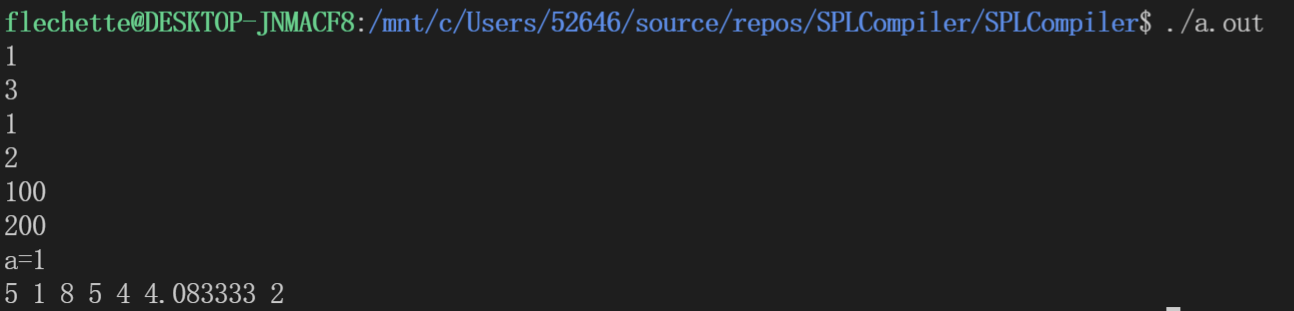
\includegraphics[width=1\textwidth]{test1res.png}
    \caption{test 1}
\end{figure}


\subsection{用例2}
\par 1+2+...+10
\subsubsection{测试代码}
\begin{lstlisting}[language=pascal,showstringspaces=false]
program hello;
var
	i : integer;

function go(a : integer): integer;
begin
	if a = 1 then
	begin
		go := 1;
	end
	else
	begin
		if a = 2 then
		begin
			go := 1;
		end
		else
		begin
			go := go(a - 1) + go(a - 2);
		end
		;
	end
	;
end
;

begin
	i := go(10);
	writeln(i);
end
.
\end{lstlisting}

\subsubsection{抽象语法树}
\begin{lstlisting}
  Program hello
  Routine
    RoutineHead
      VarDeclList
        VarDecl (i,) integer
          NameList ( i )
          SimpleTypePlain integer
      RoutinePart
        FuncDecl
          FuncHead go
            ParaDeclList
              ParaTypeList (a,) integer
                ValParaList (a,)
                SimpleTypePlain integer
            SimpleTypePlain integer
          SubRoutine
            RoutineHead
            CompoundStmt
              StmtList
                IfStmt
                  Operator ==
                    Operand Variable a
                    Operand Literal 1
                      ConstInteger 1
                  CompoundStmt
                    StmtList
                      AssignStmtSimpleType go
                        Operand Literal 1
                          ConstInteger 1
                  CompoundStmt
                    StmtList
                      IfStmt
                        Operator ==
                          Operand Variable a
                          Operand Literal 2
                            ConstInteger 2
                        CompoundStmt
                          StmtList
                            AssignStmtSimpleType go
                              Operand Literal 1
                                ConstInteger 1
                        CompoundStmt
                          StmtList
                            AssignStmtSimpleType go
                              Operator +
                                Operand Function go
                                  ArgList size 1
                                    Operator -
                                      Operand Variable a
                                      Operand Literal 1
                                        ConstInteger 1
                                Operand Function go
                                  ArgList size 1
                                    Operator -
                                      Operand Variable a
                                      Operand Literal 2
                                        ConstInteger 2
    CompoundStmt
      StmtList
        AssignStmtSimpleType i
          Operand Function go
            ArgList size 1
              Operand Literal 10
                ConstInteger 10
        SysProcStmt writeln
          ArgList size 1
            Operand Variable i
\end{lstlisting}

\subsubsection{中间码}
\begin{lstlisting}[language=LLVM]
; ModuleID = './test/test2.spl'
source_filename = "./test/test2.spl"

@i = internal global i32 0
@0 = private unnamed_addr constant [4 x i8] c"%d\0A\00", align 1

define i32 @main() {
entry:
  %go_ret = call i32 @go(i32 10)
  store i32 %go_ret, i32* @i, align 4
  %0 = call i32 (i8*, ...) @printf(i8* nonnull dereferenceable(1) getelementptr inbounds ([4 x i8], [4 x i8]* @0, i64 0, i64 0), i32 %go_ret)
  ret i32 0
}

define internal i32 @go(i32 %a) {
go_entry:
  %a1 = alloca i32, align 4
  store i32 %a, i32* %a1, align 4
  %a.off = add i32 %a, -1
  %switch = icmp ult i32 %a.off, 2
  br i1 %switch, label %ifcont12, label %else7

else7:                                            ; preds = %go_entry
  %sub = add i32 %a, -1
  %go_ret = call i32 @go(i32 %sub)
  %sub10 = add i32 %a, -2
  %go_ret11 = call i32 @go(i32 %sub10)
  %add = add i32 %go_ret11, %go_ret
  br label %ifcont12

ifcont12:                                         ; preds = %go_entry, %else7
  %storemerge14 = phi i32 [ %add, %else7 ], [ 1, %go_entry ]
  ret i32 %storemerge14
}

declare i32 @printf(i8*, ...)

\end{lstlisting}

\subsubsection{运行结果}
\begin{figure}[H]
    \centering
    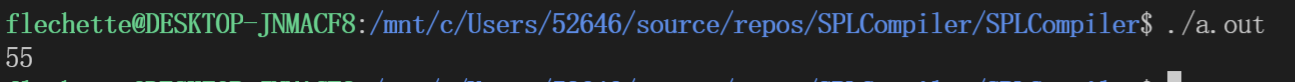
\includegraphics[width=1\textwidth]{test2res.png}
    \caption{test 2}
\end{figure}


\subsection{用例3}
\par 系统函数测试
\subsubsection{测试代码}
\begin{lstlisting}[language=pascal,showstringspaces=false]
program sysfunctest;
var
	i : integer;
	r : real;
	c : char;
begin
	read(i);
	writeln(abs(i));

	read(i);
	writeln(chr(i));

	c := 'm';
	writeln(ord(c));

	read(i);
	writeln(odd(i));

	read(i);
	writeln(pred(i));
	writeln(succ(i));
	writeln(sqr(i));

	read(r);
	writeln(sqrt(r));
end
.
\end{lstlisting}

\subsubsection{抽象语法树}
\begin{lstlisting}
Program sysfunctest
  Routine
    RoutineHead
      VarDeclList
        VarDecl (i,) integer
          NameList ( i )
          SimpleTypePlain integer
        VarDecl (r,) real
          NameList ( r )
          SimpleTypePlain real
        VarDecl (c,) char
          NameList ( c )
          SimpleTypePlain char
    CompoundStmt
      StmtList
        SysProcStmt read
          ArgList size 1
            Operand Variable i
        SysProcStmt writeln
          ArgList size 1
            Operand System Function abs
              ArgList size 1
                Operand Variable i
        SysProcStmt read
          ArgList size 1
            Operand Variable i
        SysProcStmt writeln
          ArgList size 1
            Operand System Function chr
              ArgList size 1
                Operand Variable i
        AssignStmtSimpleType c
          Operand Literal 109
            ConstCharacter 109
        SysProcStmt writeln
          ArgList size 1
            Operand System Function ord
              ArgList size 1
                Operand Variable c
        SysProcStmt read
          ArgList size 1
            Operand Variable i
        SysProcStmt writeln
          ArgList size 1
            Operand System Function odd
              ArgList size 1
                Operand Variable i
        SysProcStmt read
          ArgList size 1
            Operand Variable i
        SysProcStmt writeln
          ArgList size 1
            Operand System Function pred
              ArgList size 1
                Operand Variable i
        SysProcStmt writeln
          ArgList size 1
            Operand System Function succ
              ArgList size 1
                Operand Variable i
        SysProcStmt writeln
          ArgList size 1
            Operand System Function sqr
              ArgList size 1
                Operand Variable i
        SysProcStmt read
          ArgList size 1
            Operand Variable r
        SysProcStmt writeln
          ArgList size 1
            Operand System Function sqrt
              ArgList size 1
                Operand Variable r
\end{lstlisting}

\subsubsection{中间代码}
\begin{lstlisting}[language=LLVM]
; ModuleID = './test/test3.spl'
source_filename = "./test/test3.spl"

@i = internal global i32 0
@r = internal global double 0.000000e+00
@c = internal global i8 0
@0 = private unnamed_addr constant [3 x i8] c"%d\00", align 1
@1 = private unnamed_addr constant [4 x i8] c"%d\0A\00", align 1
@2 = private unnamed_addr constant [4 x i8] c"%c\0A\00", align 1
@3 = private unnamed_addr constant [4 x i8] c"%u\0A\00", align 1
@4 = private unnamed_addr constant [4 x i8] c"%lf\00", align 1
@5 = private unnamed_addr constant [5 x i8] c"%lf\0A\00", align 1

define i32 @main() {
entry:
  %0 = call i32 (i8*, ...) @scanf(i8* getelementptr inbounds ([3 x i8], [3 x i8]* @0, i64 0, i64 0), i32* nonnull @i)
  %i = load i32, i32* @i, align 4
  %abs = call i32 @llvm.abs.i32(i32 %i, i1 false)
  %1 = call i32 (i8*, ...) @printf(i8* nonnull dereferenceable(1) getelementptr inbounds ([4 x i8], [4 x i8]* @1, i64 0, i64 0), i32 %abs)
  %2 = call i32 (i8*, ...) @scanf(i8* getelementptr inbounds ([3 x i8], [3 x i8]* @0, i64 0, i64 0), i32* nonnull @i)
  %i1 = load i32, i32* @i, align 4
  %chr = trunc i32 %i1 to i8
  %3 = call i32 (i8*, ...) @printf(i8* nonnull dereferenceable(1) getelementptr inbounds ([4 x i8], [4 x i8]* @2, i64 0, i64 0), i8 %chr)
  store i8 109, i8* @c, align 1
  %4 = call i32 (i8*, ...) @printf(i8* nonnull dereferenceable(1) getelementptr inbounds ([4 x i8], [4 x i8]* @1, i64 0, i64 0), i32 109)
  %5 = call i32 (i8*, ...) @scanf(i8* getelementptr inbounds ([3 x i8], [3 x i8]* @0, i64 0, i64 0), i32* nonnull @i)
  %i2 = load i32, i32* @i, align 4
  %6 = and i32 %i2, 1
  %odd = icmp ne i32 %6, 0
  %7 = call i32 (i8*, ...) @printf(i8* nonnull dereferenceable(1) getelementptr inbounds ([4 x i8], [4 x i8]* @3, i64 0, i64 0), i1 %odd)
  %8 = call i32 (i8*, ...) @scanf(i8* getelementptr inbounds ([3 x i8], [3 x i8]* @0, i64 0, i64 0), i32* nonnull @i)
  %i3 = load i32, i32* @i, align 4
  %pred = add i32 %i3, -1
  %9 = call i32 (i8*, ...) @printf(i8* nonnull dereferenceable(1) getelementptr inbounds ([4 x i8], [4 x i8]* @1, i64 0, i64 0), i32 %pred)
  %i4 = load i32, i32* @i, align 4
  %succ = add i32 %i4, 1
  %10 = call i32 (i8*, ...) @printf(i8* nonnull dereferenceable(1) getelementptr inbounds ([4 x i8], [4 x i8]* @1, i64 0, i64 0), i32 %succ)
  %i5 = load i32, i32* @i, align 4
  %sqr = mul i32 %i5, %i5
  %11 = call i32 (i8*, ...) @printf(i8* nonnull dereferenceable(1) getelementptr inbounds ([4 x i8], [4 x i8]* @1, i64 0, i64 0), i32 %sqr)
  %12 = call i32 (i8*, ...) @scanf(i8* getelementptr inbounds ([4 x i8], [4 x i8]* @4, i64 0, i64 0), double* nonnull @r)
  %r = load double, double* @r, align 8
  %13 = call double @llvm.sqrt.f64(double %r)
  %14 = call i32 (i8*, ...) @printf(i8* nonnull dereferenceable(1) getelementptr inbounds ([5 x i8], [5 x i8]* @5, i64 0, i64 0), double %13)
  ret i32 0
}

declare i32 @scanf(i8*, ...)

declare i32 @printf(i8*, ...)

; Function Attrs: nofree nosync nounwind readnone speculatable willreturn
declare i32 @llvm.abs.i32(i32, i1 immarg) #0

; Function Attrs: nofree nosync nounwind readnone speculatable willreturn
declare double @llvm.sqrt.f64(double) #0

attributes #0 = { nofree nosync nounwind readnone speculatable willreturn }
\end{lstlisting}

\subsubsection{运行结果}
\begin{figure}[H]
    \centering
    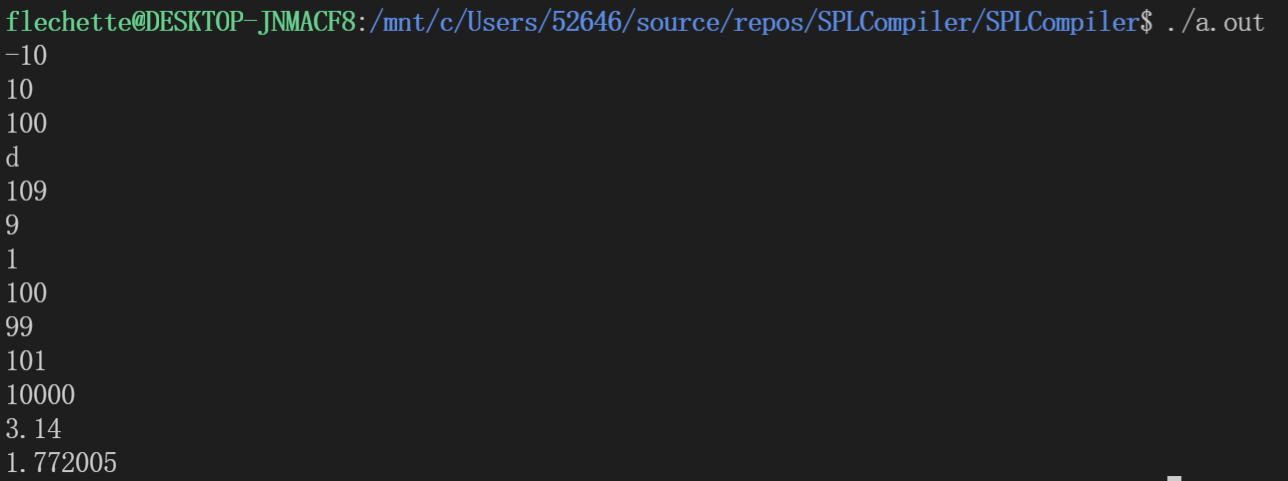
\includegraphics[width=1\textwidth]{test3res.png}
    \caption{test 3}
\end{figure}



\subsection{用例4}
\par 引用测试
\subsubsection{测试代码}
\begin{lstlisting}[language=pascal,showstringspaces=false]
program hello;
var	
	f : integer;
	k : integer;
function go(var b : integer; a : integer): integer;
var 
	fk : integer;
	t : real;

begin
	if a > 0 then 
	begin
		go := a * go(b , a - 1);
	end
	else
	begin
		go := 1;
	end
	;
	b := b + go;
	k := k + go;
end
;

begin
	k := 0;
	f := go(k , 5);
	writeln(f);
	writeln(k);
end
.
\end{lstlisting}

\subsubsection{抽象语法树}
\begin{lstlisting}
Program hello
  Routine
    RoutineHead
      VarDeclList
        VarDecl (f,) integer
          NameList ( f )
          SimpleTypePlain integer
        VarDecl (k,) integer
          NameList ( k )
          SimpleTypePlain integer
      RoutinePart
        FuncDecl
          FuncHead go
            ParaDeclList
              ParaTypeList var(b,) integer
                VarParaList var(b,)
                SimpleTypePlain integer
              ParaTypeList (a,) integer
                ValParaList (a,)
                SimpleTypePlain integer
            SimpleTypePlain integer
          SubRoutine
            RoutineHead
              VarDeclList
                VarDecl (fk,) integer
                  NameList ( fk )
                  SimpleTypePlain integer
                VarDecl (t,) real
                  NameList ( t )
                  SimpleTypePlain real
            CompoundStmt
              StmtList
                IfStmt
                  Operator >
                    Operand Variable a
                    Operand Literal 0
                      ConstInteger 0
                  CompoundStmt
                    StmtList
                      AssignStmtSimpleType go
                        Operator *
                          Operand Variable a
                          Operand Function go
                            ArgList size 2
                              Operand Variable b
                              Operator -
                                Operand Variable a
                                Operand Literal 1
                                  ConstInteger 1
                  CompoundStmt
                    StmtList
                      AssignStmtSimpleType go
                        Operand Literal 1
                          ConstInteger 1
                AssignStmtSimpleType b
                  Operator +
                    Operand Variable b
                    Operand Variable go
                AssignStmtSimpleType k
                  Operator +
                    Operand Variable k
                    Operand Variable go
    CompoundStmt
      StmtList
        AssignStmtSimpleType k
          Operand Literal 0
            ConstInteger 0
        AssignStmtSimpleType f
          Operand Function go
            ArgList size 2
              Operand Variable k
              Operand Literal 5
                ConstInteger 5
        SysProcStmt writeln
          ArgList size 1
            Operand Variable f
        SysProcStmt writeln
          ArgList size 1
            Operand Variable k
\end{lstlisting}

\subsubsection{中间代码}
\begin{lstlisting}[language=LLVM]
; ModuleID = './test/test4.spl'
source_filename = "./test/test4.spl"

@f = internal global i32 0
@k = internal global i32 0
@0 = private unnamed_addr constant [4 x i8] c"%d\0A\00", align 1

define i32 @main() {
entry:
  store i32 0, i32* @k, align 4
  %go_ret = call i32 @go(i32* nonnull @k, i32 5)
  store i32 %go_ret, i32* @f, align 4
  %0 = call i32 (i8*, ...) @printf(i8* nonnull dereferenceable(1) getelementptr inbounds ([4 x i8], [4 x i8]* @0, i64 0, i64 0), i32 %go_ret)
  %k = load i32, i32* @k, align 4
  %1 = call i32 (i8*, ...) @printf(i8* nonnull dereferenceable(1) getelementptr inbounds ([4 x i8], [4 x i8]* @0, i64 0, i64 0), i32 %k)
  ret i32 0
}

define internal i32 @go(i32* %b, i32 %a) {
go_entry:
  %a1 = alloca i32, align 4
  %go = alloca i32, align 4
  store i32 %a, i32* %a1, align 4
  %icmpsgt = icmp sgt i32 %a, 0
  br i1 %icmpsgt, label %then, label %ifcont

then:                                             ; preds = %go_entry
  %sub = add i32 %a, -1
  %go_ret = call i32 @go(i32* %b, i32 %sub)
  %mul = mul i32 %go_ret, %a
  br label %ifcont

ifcont:                                           ; preds = %go_entry, %then
  %storemerge = phi i32 [ %mul, %then ], [ 1, %go_entry ]
  store i32 %storemerge, i32* %go, align 4
  %b5 = load i32, i32* %b, align 4
  %add = add i32 %b5, %storemerge
  store i32 %add, i32* %b, align 4
  %k = load i32, i32* @k, align 4
  %add8 = add i32 %k, %storemerge
  store i32 %add8, i32* @k, align 4
  ret i32 %storemerge
}

declare i32 @printf(i8*, ...)
\end{lstlisting}

\subsubsection{运行结果}
\begin{figure}[H]
    \centering
    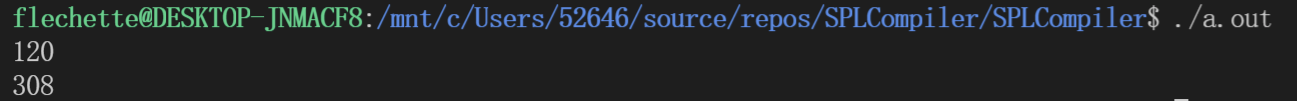
\includegraphics[width=1\textwidth]{test4res.png}
    \caption{test 4}
\end{figure}


\subsection{用例5}
\par 数组,记录的成员引用测试
\subsubsection{测试代码}
\begin{lstlisting}[language=pascal,showstringspaces=false]
program array_record_refrecursiontest;
type
	recordtype = record
		m_int: integer;
		m_double: real;
		m_bool: boolean;
	end
    ;
var
	arr : array [1..5] of integer;
    a : integer;
    i : integer;
	rec : recordtype;
    
function go(var index: integer;a : integer): integer;
begin
    index := index + 1;
	if a = 1 then
	begin
		go := 1;
	end
	else
	begin
		if a = 2 then
		begin
			go := 1;
		end
		else
		begin
			go := go(i,a - 1) + go(i,a - 2);
		end
		;
	end
	;
end
;
begin
    i := 0;
    rec.m_int := 5;
    read(arr[1]);
    a := go(i,arr[1]);
    writeln(a,' ',i);
    read(rec.m_int);
    a := go(i,rec.m_int);
    writeln(a,' ',i);
end
.
\end{lstlisting}

\subsubsection{抽象语法树}

\par 太长了,略

\subsubsection{中间代码}
\begin{lstlisting}[language=LLVM]
; ModuleID = './test/test5.spl'
source_filename = "./test/test5.spl"

@arr = internal global [5 x i32] zeroinitializer
@a = internal global i32 0
@i = internal global i32 0
@rec = internal global { i32, double, i1 } zeroinitializer
@0 = private unnamed_addr constant [3 x i8] c"%d\00", align 1
@1 = private unnamed_addr constant [8 x i8] c"%d%c%d\0A\00", align 1

define i32 @main() {
entry:
  store i32 0, i32* @i, align 4
  store i32 5, i32* getelementptr inbounds ({ i32, double, i1 }, { i32, double, i1 }* @rec, i64 0, i32 0), align 16
  %0 = call i32 (i8*, ...) @scanf(i8* getelementptr inbounds ([3 x i8], [3 x i8]* @0, i64 0, i64 0), i32* getelementptr inbounds ([5 x i32], [5 x i32]* @arr, i64 0, i64 1))
  %1 = load i32, i32* getelementptr inbounds ([5 x i32], [5 x i32]* @arr, i64 0, i64 1), align 4
  %go_ret = call i32 @go(i32* nonnull @i, i32 %1)
  store i32 %go_ret, i32* @a, align 4
  %i = load i32, i32* @i, align 4
  %2 = call i32 (i8*, ...) @printf(i8* nonnull dereferenceable(1) getelementptr inbounds ([8 x i8], [8 x i8]* @1, i64 0, i64 0), i32 %go_ret, i8 32, i32 %i)
  %3 = call i32 (i8*, ...) @scanf(i8* getelementptr inbounds ([3 x i8], [3 x i8]* @0, i64 0, i64 0), i32* getelementptr inbounds ({ i32, double, i1 }, { i32, double, i1 }* @rec, i64 0, i32 0))
  %4 = load i32, i32* getelementptr inbounds ({ i32, double, i1 }, { i32, double, i1 }* @rec, i64 0, i32 0), align 16
  %go_ret1 = call i32 @go(i32* nonnull @i, i32 %4)
  store i32 %go_ret1, i32* @a, align 4
  %i3 = load i32, i32* @i, align 4
  %5 = call i32 (i8*, ...) @printf(i8* nonnull dereferenceable(1) getelementptr inbounds ([8 x i8], [8 x i8]* @1, i64 0, i64 0), i32 %go_ret1, i8 32, i32 %i3)
  ret i32 0
}

define internal i32 @go(i32* %index, i32 %a) {
go_entry:
  %a1 = alloca i32, align 4
  store i32 %a, i32* %a1, align 4
  %index2 = load i32, i32* %index, align 4
  %add = add i32 %index2, 1
  store i32 %add, i32* %index, align 4
  %a.off = add i32 %a, -1
  %switch = icmp ult i32 %a.off, 2
  br i1 %switch, label %ifcont14, label %else8

else8:                                            ; preds = %go_entry
  %sub = add i32 %a, -1
  %go_ret = call i32 @go(i32* nonnull @i, i32 %sub)
  %sub11 = add i32 %a, -2
  %go_ret12 = call i32 @go(i32* nonnull @i, i32 %sub11)
  %add13 = add i32 %go_ret12, %go_ret
  br label %ifcont14

ifcont14:                                         ; preds = %go_entry, %else8
  %storemerge16 = phi i32 [ %add13, %else8 ], [ 1, %go_entry ]
  ret i32 %storemerge16
}

declare i32 @scanf(i8*, ...)

declare i32 @printf(i8*, ...)
\end{lstlisting}

\subsubsection{运行结果}
\begin{figure}[H]
    \centering
    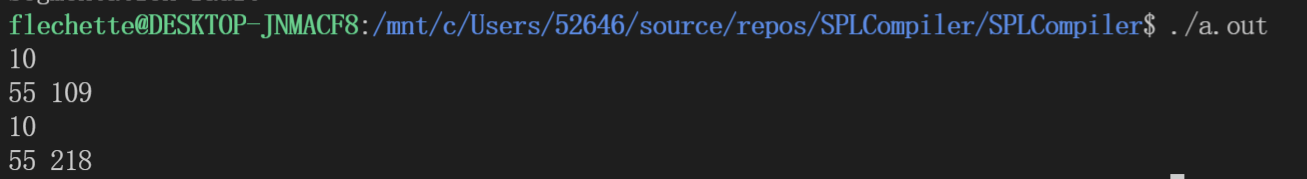
\includegraphics[width=1\textwidth]{test5res.png}
    \caption{test 5}
\end{figure}

\subsection{用例6}
\subsubsection{测试代码}
\begin{lstlisting}[language=pascal,showstringspaces=false]
program hello;
var 
	ans : integer;

function gcd(a, b : integer) : integer;
begin
	if b = 0 then begin
		gcd := a;
	end
	else begin
		gcd := gcd(b , a % b);
	end
	;
end
;

begin
	ans := gcd(9 , 36) * gcd(3 , 6);
	writeln(ans);
end
.
\end{lstlisting}
\subsubsection{抽象语法树}
\begin{lstlisting}
Program hello
  Routine
    RoutineHead
      VarDeclList
        VarDecl (ans,) integer
          NameList ( ans )
          SimpleTypePlain integer
      RoutinePart
        FuncDecl
          FuncHead gcd
            ParaDeclList
              ParaTypeList (a,b,) integer
                ValParaList (a,b,)
                SimpleTypePlain integer
            SimpleTypePlain integer
          SubRoutine
            RoutineHead
            CompoundStmt
              StmtList
                IfStmt
                  Operator ==
                    Operand Variable b
                    Operand Literal 0
                      ConstInteger 0
                  CompoundStmt
                    StmtList
                      AssignStmtSimpleType gcd
                        Operand Variable a
                  CompoundStmt
                    StmtList
                      AssignStmtSimpleType gcd
                        Operand Function gcd
                          ArgList size 2
                            Operand Variable b
                            Operator %
                              Operand Variable a
                              Operand Variable b
    CompoundStmt
      StmtList
        AssignStmtSimpleType ans
          Operator *
            Operand Function gcd
              ArgList size 2
                Operand Literal 9
                  ConstInteger 9
                Operand Literal 36
                  ConstInteger 36
            Operand Function gcd
              ArgList size 2
                Operand Literal 3
                  ConstInteger 3
                Operand Literal 6
                  ConstInteger 6
        SysProcStmt writeln
          ArgList size 1
            Operand Variable ans
\end{lstlisting}

\subsubsection{中间代码}
\begin{lstlisting}[language=LLVM]
; ModuleID = './test/test6.spl'
source_filename = "./test/test6.spl"

@ans = internal global i32 0
@0 = private unnamed_addr constant [4 x i8] c"%d\0A\00", align 1

define i32 @main() {
entry:
  %gcd_ret = call i32 @gcd(i32 9, i32 36)
  %gcd_ret1 = call i32 @gcd(i32 3, i32 6)
  %mul = mul i32 %gcd_ret1, %gcd_ret
  store i32 %mul, i32* @ans, align 4
  %0 = call i32 (i8*, ...) @printf(i8* nonnull dereferenceable(1) getelementptr inbounds ([4 x i8], [4 x i8]* @0, i64 0, i64 0), i32 %mul)
  ret i32 0
}

define internal i32 @gcd(i32 %a, i32 %b) {
gcd_entry:
  %b2 = alloca i32, align 4
  %a1 = alloca i32, align 4
  store i32 %a, i32* %a1, align 4
  store i32 %b, i32* %b2, align 4
  %icmpeq = icmp eq i32 %b, 0
  br i1 %icmpeq, label %ifcont, label %else

else:                                             ; preds = %gcd_entry
  %srem = srem i32 %a, %b
  %gcd_ret = call i32 @gcd(i32 %b, i32 %srem)
  br label %ifcont

ifcont:                                           ; preds = %gcd_entry, %else
  %storemerge = phi i32 [ %gcd_ret, %else ], [ %a, %gcd_entry ]
  ret i32 %storemerge
}

declare i32 @printf(i8*, ...)
\end{lstlisting}
\subsubsection{运行结果}
\begin{figure}[H]
    \centering
    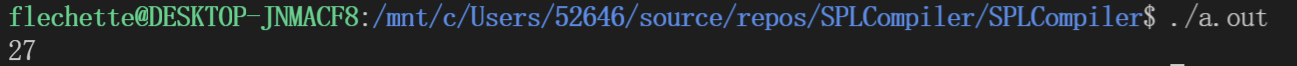
\includegraphics[width=1\textwidth]{test6res.png}
    \caption{test 6}
\end{figure}

\end{document}
